\chapter{EVALUATION, RESULTS AND OUR CONTRIBUTION }\label{our_work}

The most important part of our study is to implement these models we have examined and to make comparisons of these models after the implementation. While implementing these models, we basically used the python software language, but we also used many different libraries and frameworks. The main 2 libraries we used are pytorch and tensorflow. However, we also used libraries like matplotlib, openCV, and numpy. The structures and codes we use can be accessed on the internet in an open source manner.
\newline
Implementing Deep Learning models is always a challenge. For this purpose, we used frameworks that allow us to use graphic cards for training and test phases. Similar to all studies on inpainting we used places2 dataset \cite{dataset_places} for training and test. However due to high computational power and relatively weak GPUs we had, we needed to decrase the size of the dataset we used. An example batch from places2 dataset is shown in figure \ref{fig:dataset}

\begin{figure}[h!]
    \centering
    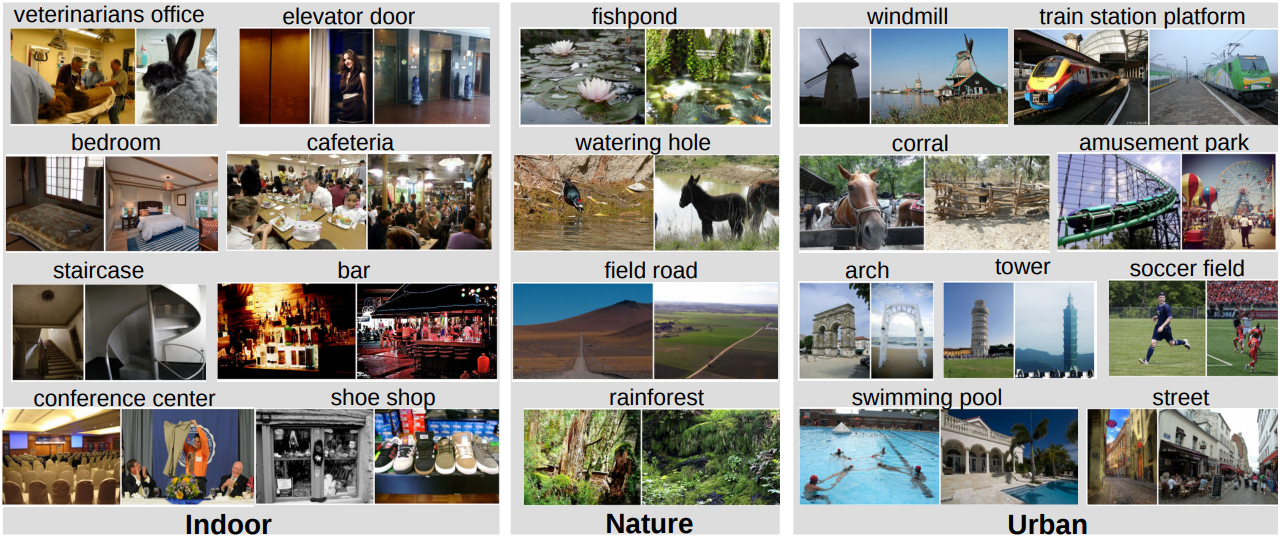
\includegraphics[scale=0.45]{figures/chapter5/Places2Dataset.PNG}
    \vspace*{4mm}
    \caption{Places2 Dataset \cite{dataset_places}}
    \label{fig:dataset}
\end{figure}

Example visual results and mathematical results over a validation dataset for different types of masks are represented in the following sections.  

\section{Framework}

One of the key points in our study was to create a model that allows many different models to work together. In order to achieve this, we had to create a framework that is easily accessible by different models and consists of parts that generate standard types of feedback. In this way, we would have obtained a modular structure where it is easy to make changes and incorporate new ideas. General structure of our framework is shown in Figure \ref{fig:framework}.

\begin{figure}[h!]
    \centering
    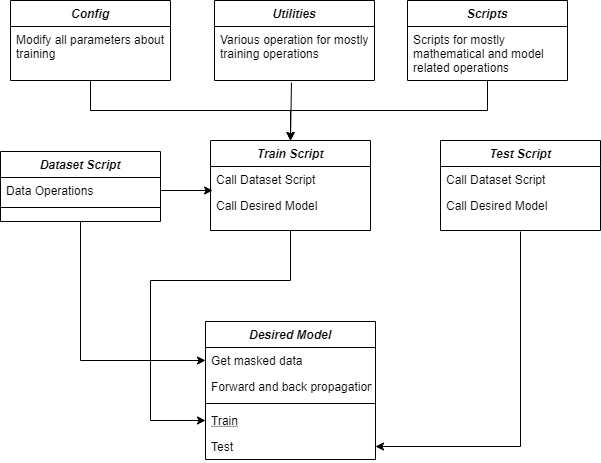
\includegraphics[scale=0.55]{figures/chapter5/framework (1).png}
    \vspace*{4mm}
    \caption{Framework}
    \label{fig:framework}
\end{figure}
In order to provide these, we created scripts that will serve as small building blocks. The most important of these building blocks are the dataset and utilities scripts, which are also actively used by models and can include important features of the models.
\newline
Masked images or transformed images that models use as input are also generated by the dataset script. We created 2 different types of masking. The first masking type we have created is the masking type that creates scattered lines on the picture which we call line masking. With this masking type, we are able to simulate smaller imperfections rather than large missing regions in the picture. Line masking example is shown in figure \ref{fig:linemasking}.

\begin{figure}[!ht]
    \centering
        \subfloat[Image]{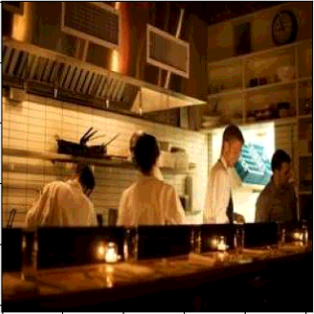
\includegraphics[width=0.3\columnwidth]{figures/chapter5/maskingtypes/line1.PNG}}
        \hspace{0.02\columnwidth}
        \subfloat[Mask]{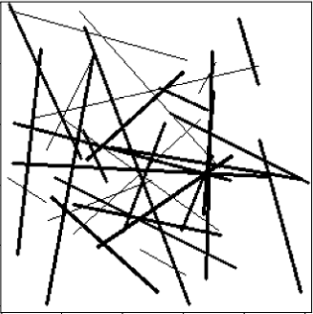
\includegraphics[width=0.3\columnwidth]{figures/chapter5/maskingtypes/line2.PNG}}
        \hspace{0.02\columnwidth}
        \subfloat[Masked Image]{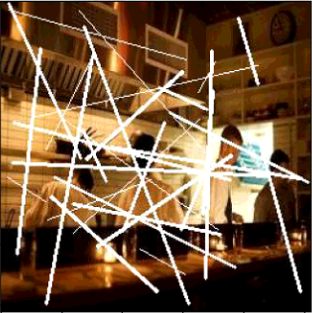
\includegraphics[width=0.3\columnwidth]{figures/chapter5/maskingtypes/line3.PNG}}
    \vspace*{3mm}
    \caption{Line Masking Example}
    \label{fig:linemasking}
\end{figure}

The other masking function we use is a function that masks a region of the given ratio value, starting from a random point on the picture. We preferred to use this masking type more to show that generative models are more successful. Our second masking type is presented in figure \ref{fig:percentagemasing}.

\begin{figure}[!ht] 
    \centering
        \subfloat[Image]{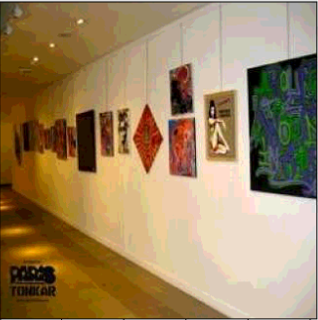
\includegraphics[width=0.3\columnwidth]{figures/chapter5/maskingtypes/percentage1.PNG}}
        \hspace{0.02\columnwidth}
        \subfloat[Mask]{
\includegraphics[width=0.3\columnwidth]{figures/chapter5/maskingtypes/percentage2.PNG}}
        \hspace{0.02\columnwidth}
        \subfloat[Masked Image]{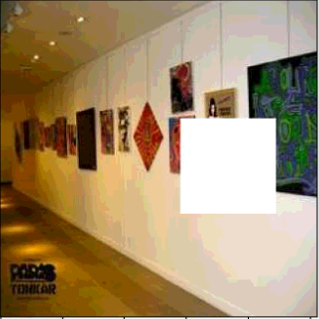
\includegraphics[width=0.3\columnwidth]{figures/chapter5/maskingtypes/percentage3.PNG}}
    \vspace*{3mm}
    \caption{Percentage Masking Example}
    \label{fig:percentagemasing}
\end{figure}

Image inpainting, unfortunately, is not a method whose success can be fully controlled with mathematical criterias. However, PSNR and SSIM values will be used throughout the project as a criterion in addition to achieving personal realistic results. Also for out comparisons mathmatical methods are used throughout our project. An example of image inpainting with one of our mathematical method which uses navier-strokes method is shown in Figure \ref{fig:mathmodel}.

\begin{figure}[!ht]
    \centering
        \subfloat[Input Image]{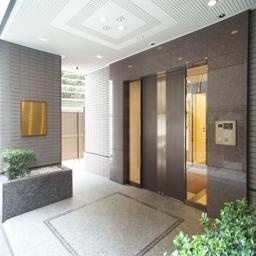
\includegraphics[width=0.3\columnwidth]{figures/chapter5/fpnvsvanilla/data1.jpg}}
        \hspace{0.02\columnwidth}
        \subfloat[Mask]{
\includegraphics[width=0.3\columnwidth]{figures/chapter5/fpnvsvanilla/data1mask.png}}
        \hspace{0.02\columnwidth}
        \subfloat[Navier-Strokes Output]{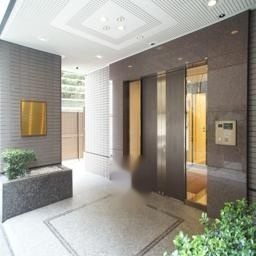
\includegraphics[width=0.3\columnwidth]{figures/chapter5/mathmodel/mathdata1.png}}
        \hspace{0.02\columnwidth}
        \subfloat[Input Image]{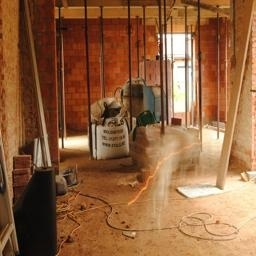
\includegraphics[width=0.3\columnwidth]{figures/chapter5/fpnvsvanilla/data2.jpg}}
        \hspace{0.02\columnwidth}
        \subfloat[Mask]{
\includegraphics[width=0.3\columnwidth]{figures/chapter5/fpnvsvanilla/data2mask.png}}
        \hspace{0.02\columnwidth}
        \subfloat[Navier-Strokes Output]{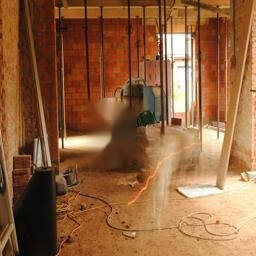
\includegraphics[width=0.3\columnwidth]{figures/chapter5/mathmodel/mathdata2.png}}
        \vspace*{3mm}
        \caption{Mathematical Model Example}
    \label{fig:mathmodel}
\end{figure}

\section{Our Contribution}

\subsection{Unified Contextual-Edge Model}
During our literature review we studied a model by Yu et al. which is called Free-Form Image Inpainting with Gated Convolution \cite{freeform_inpainting}. In this model, there are 3 main stages as shown in the Figure \ref{fig:freeform}.

\begin{figure}[h!]
    \centering
    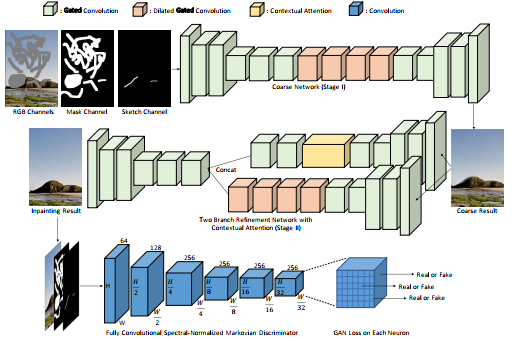
\includegraphics[scale=0.5]{figures/chapter5/Free-form.PNG}
    \vspace*{3mm}
    \caption{Free-form Image Inpainting Example \cite{freeform_inpainting}}
    \label{fig:freeform}
\end{figure}

Based on this, we wanted to try EdgeConnect and Generative Contextual Attention models in a cascaded network. Hence, there will be 3 steps in the new model. Which consists of following steps. figure \ref{fig:unifiedIdeda} shows the steps of this model. 


\begin{figure}[h!]
    \centering
    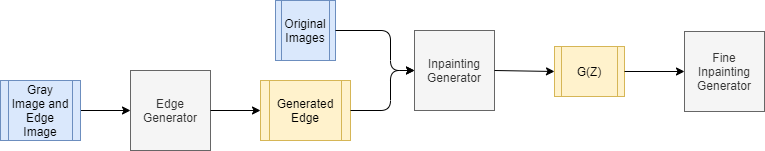
\includegraphics[scale=0.5]{figures/chapter5/Unified.png}
    \vspace*{3mm}
    \caption{Unified Model Structure }
    \label{fig:unifiedIdeda}
\end{figure}

•	Edge information prediction \newline
•	Inpainting operation with edge and RGB image as input \newline
•	Refinement network  \newline
We were able to implement this idea. However, size of the model is nearly doubled and training time is significantly increased, but it was also possible to use independently trained parameters for our models. Figure \ref{fig:unifiedexample} shows the obtained result with unified model.

\begin{figure}[!ht]
    \centering
        \subfloat[Input Image]{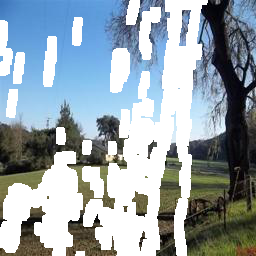
\includegraphics[width=0.45\columnwidth]{figures/chapter5/inputs/places2_05.png}}
        \hspace{0.05\columnwidth}
        \subfloat[Inpainted Image]{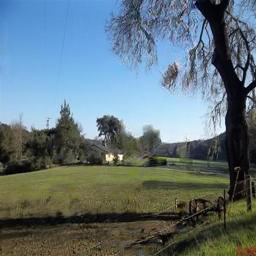
\includegraphics[width=0.45\columnwidth]{figures/chapter5/UnifiedOutput/places2_05.png}}
        \hspace{0.05\columnwidth}
        \subfloat[Input Image]{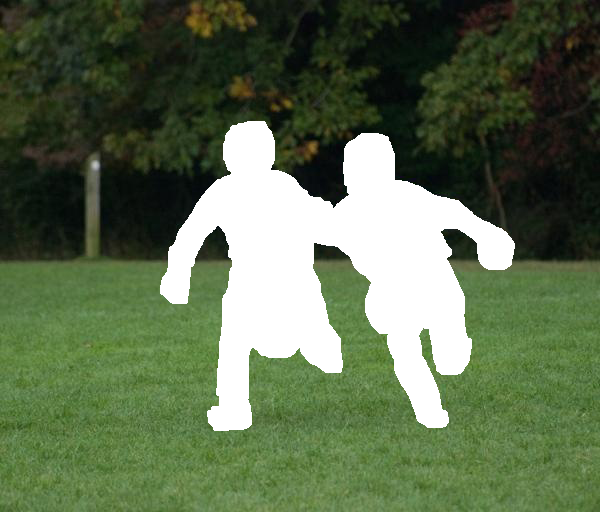
\includegraphics[width=0.45\columnwidth]{figures/chapter5/inputs/places2_06.png}}
        \hspace{0.05\columnwidth}
        \subfloat[Inpainted Image]{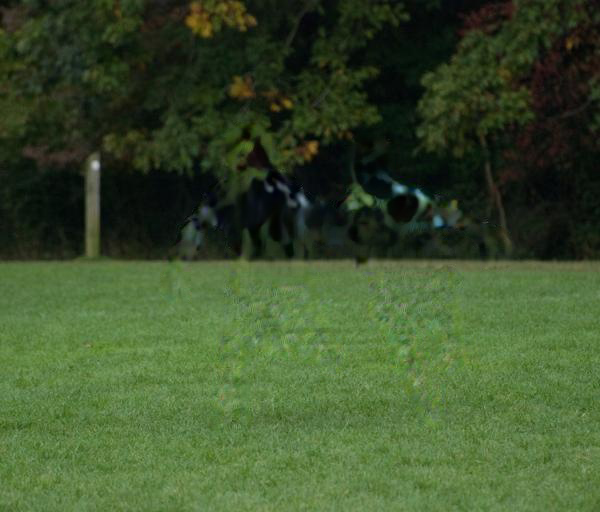
\includegraphics[width=0.45\columnwidth]{figures/chapter5/UnifiedOutput/places2_06.png}}
        \vspace*{3mm}
        \caption{Unified Model Inpainting Example}
    \label{fig:unifiedexample}
\end{figure}

\subsection{Feature Pyramid GAN Model}
Feature Pyramid Networks is proposed in paper Feature Pyramid Networks for Object Detection \cite{feature_pyramid}. FPN is commonly used in object detection problem. The basic idea behind FPN is to combine the feature information of different sizes of the same image to obtain a more inferential output. During the execution of the model, the input image is inserted into downsampling layers. The results obtained from each stage are re-included in the upsampling process in a horizontal way. Different versions of feature structures in object detection are given in \ref{fig:fpnstructs}

\begin{figure}[!ht]
    \centering
        \subfloat[Featurized Image Pyramid]{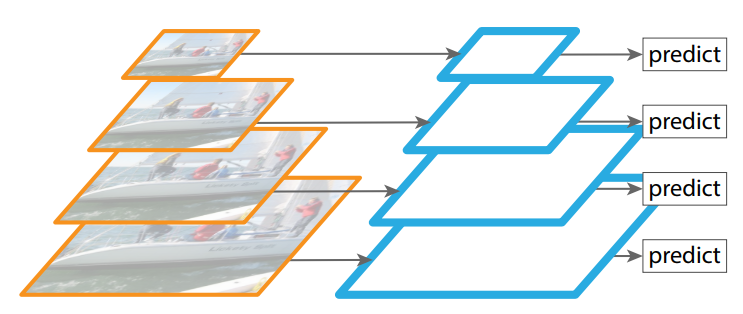
\includegraphics[width=0.45\columnwidth]{figures/chapter5/fpn1.PNG}}
        \hspace{0.05\columnwidth}
        \subfloat[Single Feature Map]{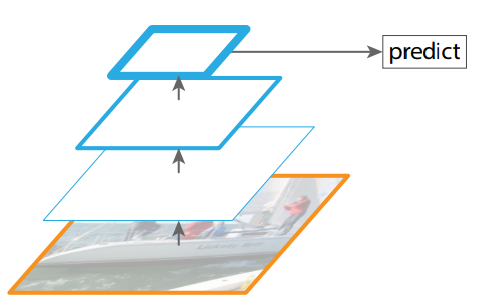
\includegraphics[width=0.4\columnwidth]{figures/chapter5/fpn2.PNG}}
        \hspace{0.05\columnwidth}
        \subfloat[Pyramidal feature hiearchy]{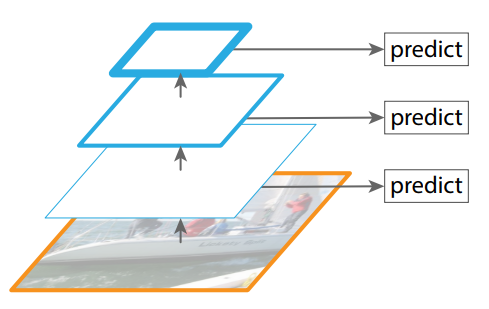
\includegraphics[width=0.4\columnwidth]{figures/chapter5/fpn3.PNG}}
        \hspace{0.05\columnwidth}
        \subfloat[Feature Pyramid Network]{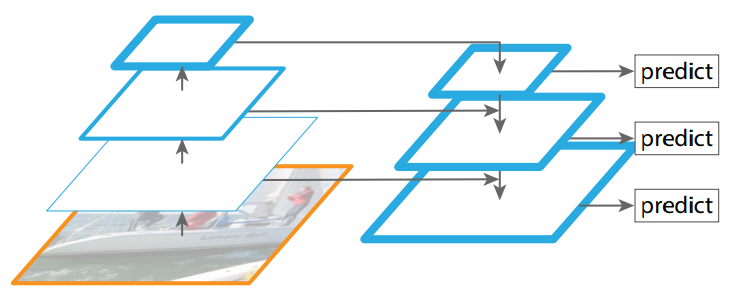
\includegraphics[width=0.45\columnwidth]{figures/chapter5/fpn4.PNG}}
        \vspace*{3mm}
        \caption{Unified Model Inpainting Example \cite{feature_pyramid}}
    \label{fig:fpnstructs}
\end{figure}

In the models we use throughout this project uses single feature map structure given in figure \ref{fig:fpnstructs}. We wanted to try out this proposed feature pyramid network for inpainting. For this purpose, a GAN model for inpainting is created which is similar to the one that is used in EdgeConnect\cite{edgeconnect} and Generative Contextual\cite{generative_contextual} models. However, generative networks of this GAN is transformed into a feature pyramid network. For comparison purposes, we also used the same network GAN network without FPN which we call Vanilla GAN. Results of these models are given in figure \ref{fig:fpnexample}

\begin{figure}[!ht]
    \centering
        \subfloat[Input Image]{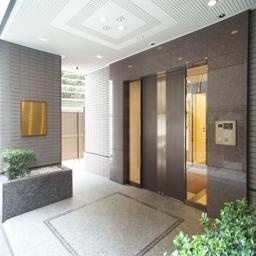
\includegraphics[width=0.22\columnwidth]{figures/chapter5/fpnvsvanilla/data1.jpg}}
        \hspace{0.02\columnwidth}
        \subfloat[Mask]{
\includegraphics[width=0.22\columnwidth]{figures/chapter5/fpnvsvanilla/data1mask.png}}
        \hspace{0.02\columnwidth}
        \subfloat[Vanilla GAN Output]{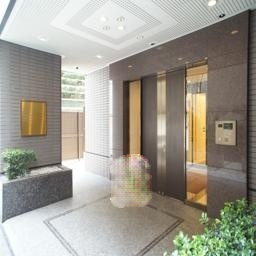
\includegraphics[width=0.22\columnwidth]{figures/chapter5/fpnvsvanilla/vandata1.png}}
        \hspace{0.02\columnwidth}
        \subfloat[FPN GAN Output]{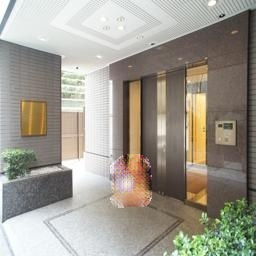
\includegraphics[width=0.22\columnwidth]{figures/chapter5/fpnvsvanilla/fpndata1.png}}
        \hspace{0.02\columnwidth}
        \subfloat[Input Image]{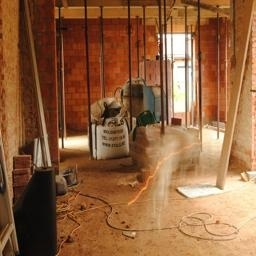
\includegraphics[width=0.22\columnwidth]{figures/chapter5/fpnvsvanilla/data2.jpg}}
        \hspace{0.02\columnwidth}
        \subfloat[Mask]{
\includegraphics[width=0.22\columnwidth]{figures/chapter5/fpnvsvanilla/data2mask.png}}
        \hspace{0.02\columnwidth}
        \subfloat[Vanilla GAN Output]{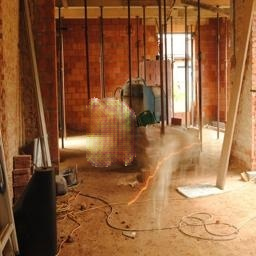
\includegraphics[width=0.22\columnwidth]{figures/chapter5/fpnvsvanilla/vandata2.png}}
        \hspace{0.02\columnwidth}
        \subfloat[FPN GGAN Output]{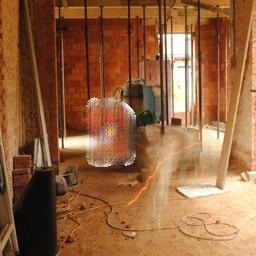
\includegraphics[width=0.22\columnwidth]{figures/chapter5/fpnvsvanilla/fpndata2.png}}
        \vspace*{3mm}
        \caption{FPN and Vanilla GAN Inpainting Example}
    \label{fig:fpnexample}
\end{figure}

\newpage
\section{Test Results}

Yazilacak.

\begin{table}[h]
\centering
\begin{tabular}{l|lllll}
\textbf{PSNR}  & Generative CNN & Contextual Attention & Unified Model      \\ \hline
10\% rectangle & 24.844490761670000  & 24.850492605756124   & 24.743092512042605 \\
20\% rectangle & 20.395097252748855  & 21.162354749478556   & 20.504682361147054 \\
random lines   & 32.143859603795630  & 31.956787492576950   & 28.981316289470524
\end{tabular}
\caption{PSNR Results}
\label{tab:PSNRresults}
\end{table}

\begin{table}[h]
\centering
\begin{tabular}{l|lllll}
\textbf{SSIM}  & Generative CNN & Contextual Attention & Unified Model      \\ \hline
10\% rectangle & 0.9061930950257007  & 0.9102801845512879   & 0.9077312745201742 \\
20\% rectangle & 0.8189780046987921  & 0.8269403263484212   & 0.8244177995307226 \\
random lines   & 0.9421359825069808  & 0.9453951610283386   & 0.9072124670658422
\end{tabular}
\caption{SSIM Results}
\label{tab:SSIMresults}
\end{table}